%%% Preliminary
% === Method Overview
\subsection{Overview}
Long-horizon manipulation relies on two contradictory capabilities: maintaining global consistency over extended history and reacting responsively to immediate dynamics. End-to-end approaches typically struggle to balance these needs—short-context policies suffer from catastrophic forgetting, while heavy reasoning models incur prohibitive latency for real-time control.

To address this challenge, we propose HiMe, a Hierarchical Embodied Memory framework that decouples embodied intelligence into three functional layers: 
(1) The Executor $\pi_e$: A high-frequency VLA that ensures physical stability by mapping immediate observations to actions. 
(2) The Sentry $\pi_s$: A lightweight VLM that identifies progress changes in the environment, triggering planning only when necessary.
(3) The Planner $\pi_p$: A heavyweight VLM that uses long-term episodic memory and plans at a lower frequency.
This separation allows the system to amortize the cost of complex planning over extended execution windows, ensuring the low-level controller remains responsive to immediate physical dynamics while maintaining long-term task coherence. 

% === Problem Formulation
\textbf{Problem Setup.} 
We formulate the long-horizon manipulation task as a sequential decision-making process under partial observability. The agent operates over a horizon $T \gg 1$, receiving high-dimensional observations $o_t \in \mathcal{O}$ and a natural language instruction $l$. The objective is to generate an action sequence $a_{0:T}$ that transitions the environment to a state satisfying the instruction $l$. Ideally, the optimal action at any step $t$ depends on the full interaction history $h_t = (o_0, a_0, \dots, o_t)$ to resolve ambiguity and track progress. However, processing $h_t$ continuously is computationally intractable. To address this, we adopt a hierarchical policy $\pi(a_t \mid o_{0:t}, l)$.

\begin{figure*}
    \centering
    
\includegraphics[width=0.85\linewidth]{imgs/hime.pdf}
    \caption{\textbf{Architecture of HiMe.} The Sentry module serves as a real-time monitor, periodically tracking the executor's progress and buffering visual observations. Upon detecting the completion of a subtask, it triggers the Planner to review the entire execution trajectory. The Planner then performs memory retrieval and consolidation to update the contextual memory and refines the procedure memory. Finally, the refined instruction is fed back to the Sentry to resume monitoring the executor, forming a robust closed-loop system. }
    \label{fig:hime}
\end{figure*}


\subsection{Hierarchical Embodied Memory}
To bridge the gap between reflexes and reflection, we augment the agent with a structured state space comprising three distinct components. This explicitly represents the information required for immediate control, temporal monitoring, and long-term planning.

\textbf{Transient Memory ($\mathcal{T}_t$).} Managed by the Executor, it contains the instantaneous observation $o_t$. It serves as the minimal sufficient state for reactive sensory-motor coordination.

\textbf{Working Memory ($\mathcal{W}_t$).} 
To support high-frequency monitoring, we maintain a sliding window of recent observations $\mathcal{W}_t = \{o_{t-h_s}, \dots, o_t\}$. Unlike the main memory, this buffer is transient and raw, capturing the immediate dynamics required for verifying subgoal status or detecting sudden failures.

\textbf{Episodic Memory ($\mathcal{E}_t$).} A persistent long-term store managed by the Planner, consisting of: 
(1) \textit{Contextual Memory $\mathcal{E}_t^{c}$} 
, a multimodal key--value store $\mathcal{M}_t$ that accumulates compact, task-relevant information—including both visual imagery and textual descriptions—over time, such as object state changes, spatial constraints, or human preferences, and supports retrieval via textual keys.
(2) \textit{Procedural Memory $\mathcal{E}_t^{p}$} 
, a structured plan $\mathcal{E}_t^{p} = \{\tau_i\}_{i=1}^{N}$ consisting of an ordered list of language subgoals, where the active subgoal $\tau_t^{(i)}$ carries status labels like `active', `pending' or `done' to synchronize the control loop.

%%% Hierarchical Embodied Memory
% \subsection{Hierarchical Policy Decomposition}
% We decompose the decision-making process into a three-tiered hierarchy. This design ranges from a memory-free execution layer to a long-horizon reasoning layer, progressively trading off frequency for context capacity.

\subsection{Hierarchical Policy Decomposition}
We decompose the hierarchical policy $\pi(a_t \mid o_{0:t}, l)$ into a three-tiered hierarchy. 
This design ranges from a memory-free execution layer to a long-horizon reasoning layer, progressively trading off frequency for context capacity, decoupling immediate actuation from high-level reasoning. Formally, the decision process at time $t$ involves interactions between a base executor $\pi_e$, a monitoring Sentry $\pi_s$, and a reasoning Planner $\pi_p$.

% % === VLA as stateless low-level controller
% \textbf{Base-level VLA Executor.}
% At the base level, we employ a VLA model as the system's actuator. Operating at the highest frequency, this policy $\pi_e$ holds no explicit memory of past events. Instead, it relies on the current execution plan $\mathcal{P}_t$ provided by the upper layers. By conditioning on the active subgoal $\tau_t^{(i)} \in \mathcal{P}_t$, $\pi_e$ maps local observations to actions. This design isolates the actuation from the complexity of long-horizon dependencies, allowing the robot to react smoothly to physical dynamics as long as the high-level guidance remains valid.
\textbf{Base-level Executor ($\pi_e$).}
At the base level, the executor functions as a high-frequency reactive policy. We assume a local Markov property where, given an active language subgoal $\tau_t \in \mathcal{E}_t^p$, the optimal action is conditionally independent of the long-term history. The executor maps the current observation and subgoal to an action:
\begin{equation}
    a_t \sim \pi_e(a_t \mid o_t, \tau_t),
\end{equation}
where $\tau_t$ serves as a conditioning variable abstracted from the complex episodic history, representing the current executing subgoal. This design ensures that $\pi_e$ remains stateless and computationally efficient, enabling real-time responsiveness to physical dynamics.

% % === Sentry for High-Frequency Progress Monitoring
\textbf{Agile Sentry ($\pi_s$).}
The second layer is the Sentry, it is a gating function $u_t \in \{0, 1\}$ that be used to amortize the computational cost of reasoning. Operating on the sliding window working memory $\mathcal{W}_t$, the Sentry evaluates subgoal completion or environmental deviation at intervals of $n_m$:
\begin{equation}
    u_t = 
    \begin{cases} 
    \mathbb{I}[\pi_s(\mathcal{W}_t, \tau_t) > \delta] & \text{if } t \equiv 0 \pmod{n_m} \\
    0 & \text{otherwise,}
    \end{cases}
\end{equation}
where $\mathbb{I}[\cdot]$ is the indicator function and $\delta$ is a decision threshold. $u_t=1$ signals a "handover" event—indicating that the current subgoal $\tau_t$ is either completed or invalidated, thereby triggering the Planner. When $u_t=0$, the system bypasses high-level reasoning, maintaining the current latent state $\mathcal{E}_{t+1} \leftarrow \mathcal{E}_t$.

% % === Planner for Low-Frequency Reasoning and Long-Horizon Memory Update
\textbf{Reasoning Planner ($\pi_p$).}
When triggered ($u_t=1$), the Planner performs a belief update on the episodic memory $\mathcal{E}_t$ to re-align the agent's internal state with the environment. This process is formulated as a two-stage transition:

(1) \textit{Context Retrieval:} The Planner first generates a query $q$ to retrieve a subset of task-relevant knowledge $\mathcal{M}_{ret} \subset \mathcal{E}_t^c$ via semantic similarity:
\begin{equation}
    q = f_{\text{enc}}(l, \mathcal{W}_t); \quad \mathcal{M}_{ret} = \text{TopK}(\mathcal{E}_t^c, q).
\end{equation}

(2) \textit{Memory Update \& Re-planning:} Conditioned on the global instruction $l$, working memory $\mathcal{W}_t$, and retrieved context $\mathcal{M}_{ret}$, the Planner updates the episodic memory state:
\begin{equation}
    (\mathcal{E}_{t+1}^c, \mathcal{E}_{t+1}^p) \leftarrow \pi_p(l, \mathcal{W}_t, \mathcal{M}_{ret}, \mathcal{E}_t^p).
\end{equation}
Specifically, this update involves symbolic operations on the Contextual Memory $\mathcal{E}^c$ to reflect new world states, and the synthesis of a new procedural plan $\mathcal{E}_{t+1}^p$. 
This involves three atomic operations: (a) \texttt{Add:} registering new environmental facts or user preferences; (b) \texttt{Update:} rectifying outdated entries; and (c) \texttt{Delete:} removing stale or conflicting data to maintain a concise representation. 
The next subgoal $\tau_{t+1}$ is then sampled from the updated plan, closing the hierarchical loop.

\begin{figure*}[t]
    \centering
    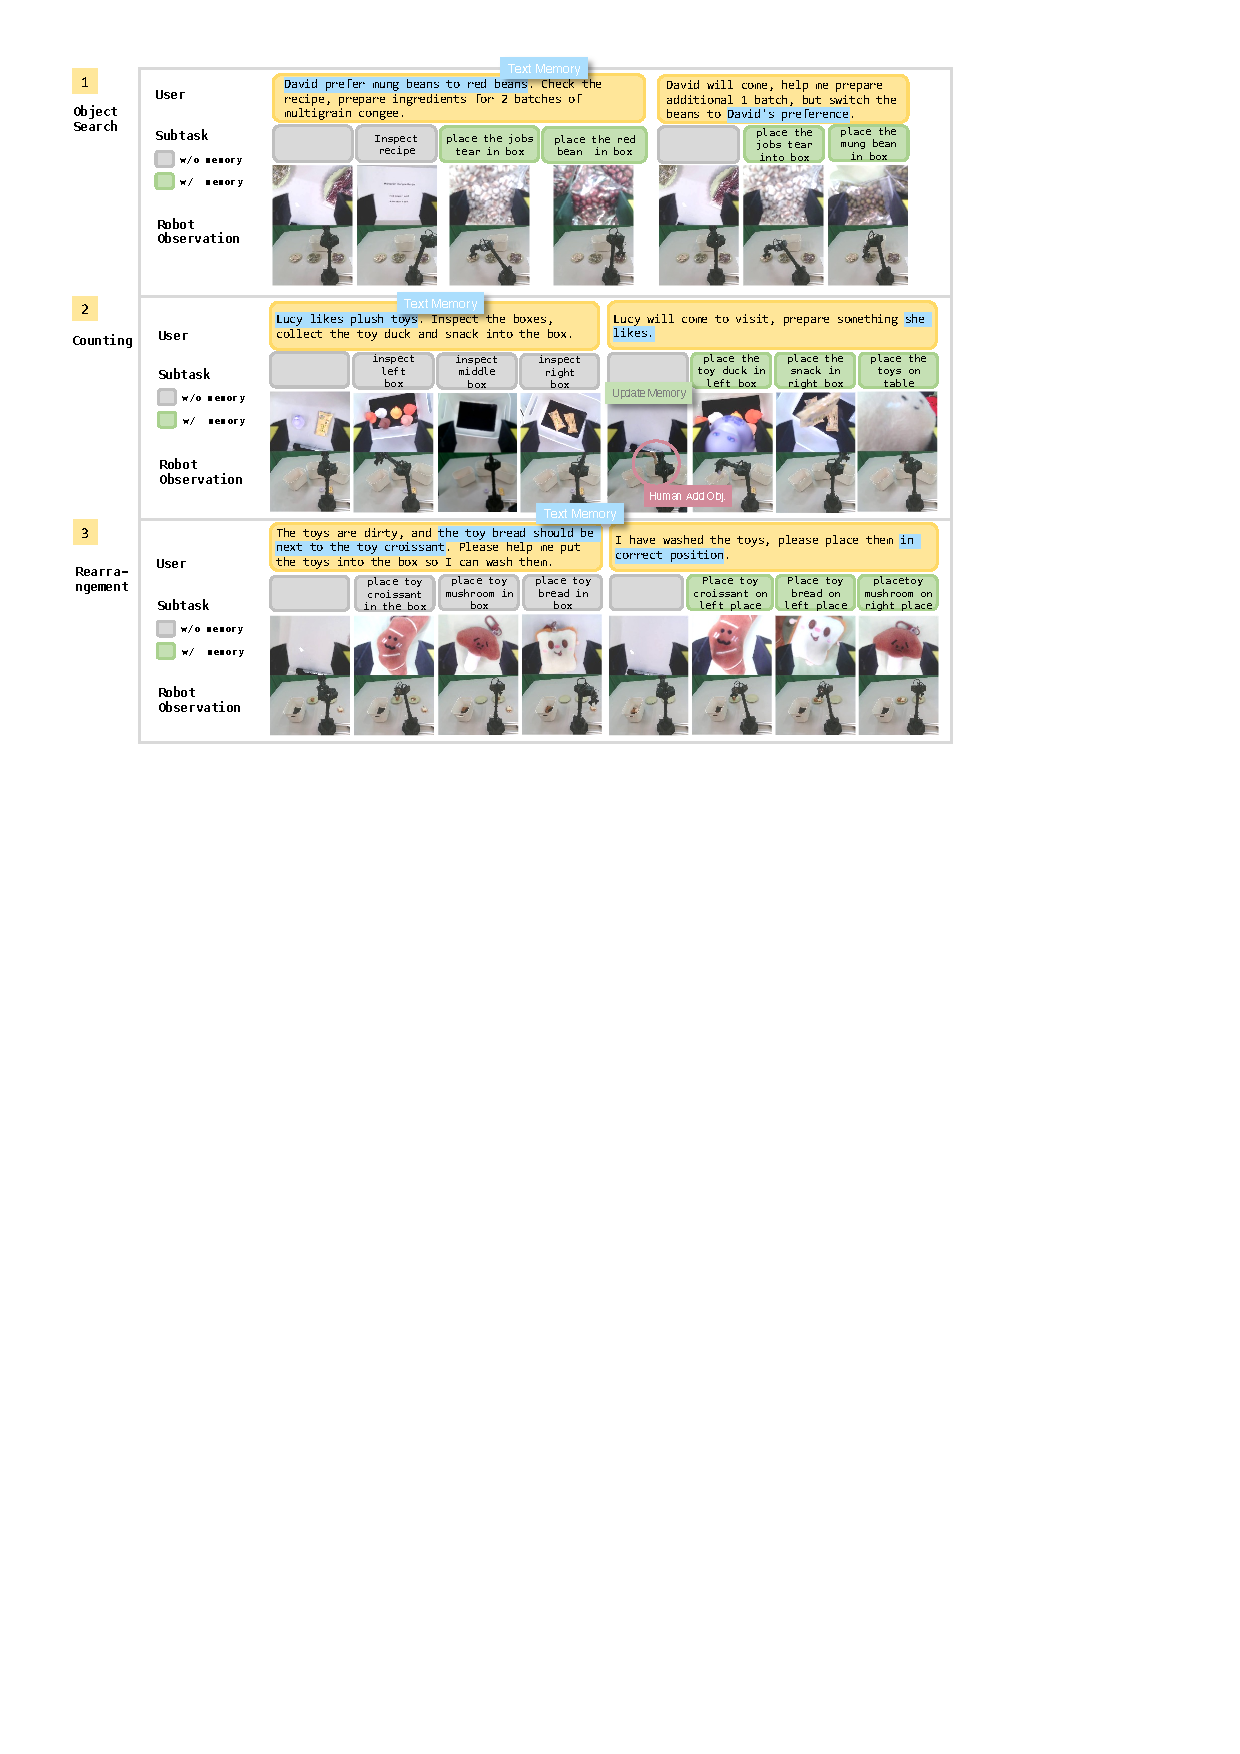
\includegraphics[width=0.98\linewidth]{imgs/exp2.pdf}
    \caption{Tasks used in our evaluations. We report performance across 20 trials per task per method.}
    \label{fig:exp}
\end{figure*}

\subsection{Implementation Details} 
While our framework is model-agnostic, we instantiate the Planner with GPT-4o~\cite{Hurst2024GPT4oSC} for its strong multimodal reasoning capabilities, and the Sentry with Qwen3-VL-8B~\cite{Bai2025Qwen3VLTR} for its balance of speed and grounding accuracy. The memory backend utilizes a vector database for semantic retrieval, utilizing OpenAI's text-embedding-3 model to encode text queries and storing multimodal memory entries alongside their caption embeddings for cosine similarity retrieval. We set the buffer size $h_s = 8$ and the monitoring interval $n_m = 5$. Consistent with our design philosophy, only the lightweight $\pi_e$, a fine-tuned VLA based on $\pi_{0.5}$, requires domain-specific training. The Sentry and Planner operate in a zero-shot or few-shot manner, leveraging pre-trained generalization to handle long-horizon logic without extensive data collection.
